%%%%%%%%%%%%%%%%%%%%%%%%%%%%%%%%%%%%%%%%%
% Programming/Coding Assignment
% LaTeX Template
%
% This template has been downloaded from:
% http://www.latextemplates.com
%
% Original author:
% Ted Pavlic (http://www.tedpavlic.com)
%
% Note:
% The \lipsum[#] commands throughout this template generate dummy text
% to fill the template out. These commands should all be removed when 
% writing assignment content.
%
% This template uses a Perl script as an example snippet of code, most other
% languages are also usable. Configure them in the "CODE INCLUSION 
% CONFIGURATION" section.
%
%%%%%%%%%%%%%%%%%%%%%%%%%%%%%%%%%%%%%%%%%

%----------------------------------------------------------------------------------------
%	PACKAGES AND OTHER DOCUMENT CONFIGURATIONS
%----------------------------------------------------------------------------------------

\documentclass{article}

\usepackage{fancyhdr} % Required for custom headers
\usepackage{lastpage} % Required to determine the last page for the footer
\usepackage{extramarks} % Required for headers and footers
\usepackage[usenames,dvipsnames]{color} % Required for custom colors
\usepackage{graphicx} % Required to insert images
\usepackage{listings} % Required for insertion of code
\usepackage{courier} % Required for the courier font
\usepackage{lipsum} % Used for inserting dummy 'Lorem ipsum' text into the template
\usepackage[T1]{fontenc}
\usepackage{amsmath, amsthm, amssymb}
\usepackage[ansinew]{inputenc}
\usepackage{pdfpages}
\usepackage{minted}
\usepackage{enumerate}
\usepackage{adjustbox}
\usepackage{bm}

% Margins
\topmargin=-0.45in
\evensidemargin=0in
\oddsidemargin=0in
\textwidth=6.5in
\textheight=9.0in
\headsep=0.25in

\linespread{1.1} % Line spacing

% Set up the header and footer
\pagestyle{fancy}
\lhead{\hmwkAuthorName} % Top left header
\chead{\hmwkClass\ \hmwkTitle} % Top center head
\rhead{\firstxmark} % Top right header
\lfoot{\lastxmark} % Bottom left footer
\cfoot{} % Bottom center footer
\rfoot{Page\ \thepage\ of\ \protect\pageref{LastPage}} % Bottom right footer
\renewcommand\headrulewidth{0.4pt} % Size of the header rule
\renewcommand\footrulewidth{0.4pt} % Size of the footer rule

\setlength\parindent{0pt} % Removes all indentation from paragraphs

%----------------------------------------------------------------------------------------
%	CODE INCLUSION CONFIGURATION
%----------------------------------------------------------------------------------------

\definecolor{MyDarkGreen}{rgb}{0.0,0.4,0.0} % This is the color used for comments
\lstloadlanguages{Perl} % Load Perl syntax for listings, for a list of other languages supported see: ftp://ftp.tex.ac.uk/tex-archive/macros/latex/contrib/listings/listings.pdf
\lstset{language=Perl, % Use Perl in this example
        frame=single, % Single frame around code
        basicstyle=\small\ttfamily, % Use small true type font
        keywordstyle=[1]\color{Blue}\bf, % Perl functions bold and blue
        keywordstyle=[2]\color{Purple}, % Perl function arguments purple
        keywordstyle=[3]\color{Blue}\underbar, % Custom functions underlined and blue
        identifierstyle=, % Nothing special about identifiers                                         
        commentstyle=\usefont{T1}{pcr}{m}{sl}\color{MyDarkGreen}\small, % Comments small dark green courier font
        stringstyle=\color{Purple}, % Strings are purple
        showstringspaces=false, % Don't put marks in string spaces
        tabsize=5, % 5 spaces per tab
        %
        % Put standard Perl functions not included in the default language here
        morekeywords={rand},
        %
        % Put Perl function parameters here
        morekeywords=[2]{on, off, interp},
        %
        % Put user defined functions here
        morekeywords=[3]{test},
       	%
        morecomment=[l][\color{Blue}]{...}, % Line continuation (...) like blue comment
        numbers=left, % Line numbers on left
        firstnumber=1, % Line numbers start with line 1
        numberstyle=\tiny\color{Blue}, % Line numbers are blue and small
        stepnumber=5 % Line numbers go in steps of 5
}

% Creates a new command to include a perl script, the first parameter is the filename of the script (without .pl), the second parameter is the caption
%%\newcommand{\perlscript}[2]{
%%\begin{itemize}
%%\item[]\lstinputlisting[caption=#2,label=#1]{#1.pl}
%%\end{itemize}
%%}

%----------------------------------------------------------------------------------------
%	DOCUMENT STRUCTURE COMMANDS
%	Skip this unless you know what you're doing
%----------------------------------------------------------------------------------------

% Header and footer for when a page split occurs within a problem environment
\newcommand{\enterProblemHeader}[1]{
\nobreak\extramarks{#1}{#1 continued on next page\ldots}\nobreak
\nobreak\extramarks{#1 (continued)}{#1 continued on next page\ldots}\nobreak
}

% Header and footer for when a page split occurs between problem environments
\newcommand{\exitProblemHeader}[1]{
\nobreak\extramarks{#1 (continued)}{#1 continued on next page\ldots}\nobreak
\nobreak\extramarks{#1}{}\nobreak
}

\setcounter{secnumdepth}{0} % Removes default section numbers
\newcounter{homeworkProblemCounter} % Creates a counter to keep track of the number of problems

\newcommand{\homeworkProblemName}{}
\newenvironment{homeworkProblem}[1][Problem \arabic{homeworkProblemCounter}]{ % Makes a new environment called homeworkProblem which takes 1 argument (custom name) but the default is "Problem #"
\stepcounter{homeworkProblemCounter} % Increase counter for number of problems
\renewcommand{\homeworkProblemName}{#1} % Assign \homeworkProblemName the name of the problem
\section{\homeworkProblemName} % Make a section in the document with the custom problem count
\enterProblemHeader{\homeworkProblemName} % Header and footer within the environment
}{
\exitProblemHeader{\homeworkProblemName} % Header and footer after the environment
}

\newcommand{\problemAnswer}[1]{ % Defines the problem answer command with the content as the only argument
\noindent\framebox[\columnwidth][c]{\begin{minipage}{0.98\columnwidth}#1\end{minipage}} % Makes the box around the problem answer and puts the content inside
}

\newcommand{\homeworkSectionName}{}
\newenvironment{homeworkSection}[1]{ % New environment for sections within homework problems, takes 1 argument - the name of the section
\renewcommand{\homeworkSectionName}{#1} % Assign \homeworkSectionName to the name of the section from the environment argument
\subsection{\homeworkSectionName} % Make a subsection with the custom name of the subsection
\enterProblemHeader{\homeworkProblemName\ [\homeworkSectionName]} % Header and footer within the environment
}{
\enterProblemHeader{\homeworkProblemName} % Header and footer after the environment
}

%----------------------------------------------------------------------------------------
%	NAME AND CLASS SECTION
%----------------------------------------------------------------------------------------

\newcommand{\hmwkTitle}{Midterm} % Assignment title
\newcommand{\hmwkDueDate}{March\ 11,\ 2016} % Due date
\newcommand{\hmwkClass}{Data Mining\ CS573} % Course/class
\newcommand{\hmwkAuthorName}{Yu-Chen Chang} % Your name

%----------------------------------------------------------------------------------------
%	TITLE PAGE
%----------------------------------------------------------------------------------------

\title{
\vspace{2in}
\textmd{\textbf{\hmwkClass:\ \hmwkTitle}}\\
\normalsize\vspace{0.1in}\small{\hmwkDueDate}\\
\vspace{3in}
}

\author{\textbf{\hmwkAuthorName}}
\date{} % Insert date here if you want it to appear below your name

%----------------------------------------------------------------------------------------

\begin{document}

\maketitle

%----------------------------------------------------------------------------------------
%	TABLE OF CONTENTS
%----------------------------------------------------------------------------------------

%\setcounter{tocdepth}{1} % Uncomment this line if you don't want subsections listed in the ToC

\newpage
\tableofcontents
\newpage

%----------------------------------------------------------------------------------------
%	PROBLEM 1
%----------------------------------------------------------------------------------------

% To have just one problem per page, simply put a \clearpage after each problem

\begin{homeworkProblem}
\begin{enumerate}[a.]
%% NBC %%
\item \ 
	\begin{enumerate}[i.]
	% a-i %
	\item Naive Bayes Classifier: \\ \\
	From the naive bayes classifier, we have the formula: \\
	$P(C|\mathbf{X}) = \frac{P(\mathbf{X}|C)P(C)}{P(\mathbf{X})} \propto P(\mathbf{X}|C)P(C)$ (Bayes rule), where C is the class random variable and \textbf{X} is the attribute random vector. \\ \\
	In NBC, there is an assumption that attributes are conditionally independent given the class, Therefore, we have the naive Bayes classifier: \\
	$P(C|\mathbf{X}) \propto P(\mathbf{X}|C)P(C) \propto \prod_{i=1}^{m}P(X_{i}|C)P(C)$ , where m is the number of attributes and $X_i$ is the $i$-th attribute random variable.\\ \\
	Because we don't know the distribution of $P(X_{i}|C)$ and $P(C)$,
	Therefore, we need likelihood function to determine unknown parameters based on known outcomes. Assume the data D are independently sampled from the same distribution. Let $D = [\mathbf{x}_1, ... , \mathbf{x}_n]$, where n is the number of samples:
	\begin{align}
	L(\theta|D) &= \prod_{i=1}^{n}P(\mathbf{x}_{i},c_{i}|\theta) \text{\ \ (general likelihood)}\\
	&\propto \prod_{i=1}^{n}P(\mathbf{x}_{i}|c_{i},\theta)P(c_i|\theta) \text{\ \ (Bayes rule)}\\ 
	&\propto \prod_{i=1}^{n} \prod_{j=1}^{m}P(x_{ij}|c_{i},\theta)P(c_i|\theta) \text{\ \ (Naive assumption)}
	\end{align}
	We apply Maximum Likelihood estimation to learn the best parameters by finding the value $\theta$ that maximizes likelihood:
	\begin{align}
	\hat{\theta}_{MLE} = arg\ \underset{\theta}{max}L(\theta)
	\end{align}
	For Multinomials, Let $A \in \{1,...,k\}$ be a discrete random variable with k values, where $P(A=j) = \theta_j$. Then P(A) is a multinomial distribution:\\
	\begin{align}
	P(A|\theta) = \prod_{j=1}^{k}\theta_{j}^{I(A=j)} \text{\ ,\ where $I(A=j)$ is an indicator function.}
	\end{align}
	The likelihood for a data set D is:
	\begin{align}
	P(D|\theta) = \prod_{i=1}^{n}\prod_{j=1}^{k}\theta_{j}^{I(A=j)} = \prod_{j}\theta_i^{n_j}
	\end{align}
	Therefore, by using Lagrange multipliers, the maximum likelihood estimates for each parameter are:
	\begin{align}
	\hat{\theta_j} = \frac{n_j}{n}
	\end{align}
	which means that in multinomial case, MLE can be determined analytically by counting. \\ \\
	For continuous inputs $X_i$, the common way to represent the distributions $P(X_i|Y)$ to assume that for each possible discrete value $y_k$ of Y, the distribution of each continuous $X_i$ is Gaussian, and is defined by a mean and standard deviation specific to $X_i$ and $y_k$.
	\begin{align}
	\mu_{ik} &= E[X_i|Y=y_k] \\
	\sigma_{ik}^{2} &= E[(X_i-\mu_{ik})^2|Y=y_k] 
	\end{align}
	Again, by MLE, we get: \\
	\begin{align}
	\hat\mu_{ik} &= \frac{1}{\sum_{j}\delta(Y^j=y_k)}\sum_{j}X_i^j\delta(Y^j=y_k) \\
	\hat\sigma_{ik}^{2} &= \frac{1}{\sum_{j}\delta(Y^j=y_k)}\sum_{j}(X_i^j-\hat{\mu_{ik}})^2\delta(Y^j=y_k)
	\end{align}
	Then we can estimate continuous attributes using Gaussian distribution with $\hat\mu_{ik}$ and $\hat\sigma_{ik}^{2}$. \\
	
	In this question, we are given 11 attributes.
	\begin{enumerate}[1.]
	\item Record Number
	\item Amount Requested
	\item Interest Rate Percentage
	\item Loan Length in Months
	\item Loan Title
	\item Loan Purpose
	\item Monthly Payment
	\item Total Amount Funded
	\item Debt-To-Income Ratio Percentage
	\item FICO Range
	\item Status
	\end{enumerate}
	The Record Number is used as id and will not be considered as an attribute and Status is the classification goal that we are interested in and used as the class random variable. Therefore, the potential attributes are from the 2 to 10 entry, which forms our attribute random vector. \\ \\
	In the step of classifying out-of-sample items, we will use the above shown formula to calculate the P(C|X) and compare $P(C=c_1|X)$ with $P(C=c_2|X)$ to see whether the out-of-sample with its attributes given in X should belong to $c_1$ or $c_2$ class.
	% a-ii %
	\item From the MLE, we have the formula 
	\begin{align}
	\hat{\theta_j} = \frac{n_j}{n}
	\end{align}
	The prior is estimated from the dataset by counting the number of each class among the entire dataset. However, if the real value prior is far from the estimated one, it will have significant impacts on the correctness of the prediction. For example, if we have a dataset with half of people with cancer and other half are healthy while in really life the probability that a person has a cancer is nearly 0.01\%, then in this situation the prior will be estimated wrong (50\%), which should be 0.01\% for cancer class and 99.99\% for healthy class, and cause large false positive in this prediction. Therefore, we can see that the wrong prior in NBC will cause either false positive or false negative to increase depending on the difference between real prior and the estimated one. That's the reason why prior in NBC is important. 
	\end{enumerate}
\clearpage
%% Logistic Regression %%
\item Logistic Regression: \\
	% b-i %
	\begin{enumerate}[i.]
	\item
	In logistic regression, we make the assumption that
	\begin{align}
	log\frac{P(\mathbf{x},y=1)}{P(\mathbf{x},y=0)} = \mathbf{w}^T\mathbf{x} + w_0
	\end{align}
	which is equivalent to 
	\begin{align}
	P(y=1|\mathbf{x}) &= \frac{1}{1+e^{-(\mathbf{w}^T\mathbf{x}+w_0)}} \\
	P(y=0|\mathbf{x}) &= \frac{e^{-(\mathbf{w}^T\mathbf{x}+w_0)}}{1+e^{-(\mathbf{w}^T\mathbf{x}+w_0)}}
	\end{align}
	Using the canonical representation of the data (adding a dummy feature of value 1 to each input vector), we have
	\begin{align}
	P(y=1|\mathbf{x}) &= g(\mathbf{x},\mathbf{w})= \frac{1}{1+e^{-\mathbf{w}^T\mathbf{x}}} \\
	P(y=0|\mathbf{x}) &= 1-g(\mathbf{x},\mathbf{w}) = \frac{e^{-\mathbf{w}^T\mathbf{x}}}{1+e^{-\mathbf{w}^T\mathbf{x}}}
	\end{align}
	These equations mean that given a training data set $\{(\mathbf{x}_i,y_i):i=1,...,N\}$, and $\mathbf{x}_i \in R^{d+1}$, where N is the total number of training examples and d is the original feature dimension, the learning goal is to find the optimal weight vector $\mathbf{w}$. \\
	The next step is to learn the parameters by using MLE. The log likelihood function is as follows:
	\begin{align}
	L(\mathbf{w}) = \sum_{i=1}^{N}log\ p(y_i|\mathbf{x}_i) = \sum_{i=1}^{N}log\ g(\mathbf{x}_i,\mathbf{w})^{y_i}(1-g(\mathbf{x}_i,\mathbf{w}))^{1-y_i}
	\end{align}
	Taking gradient of L with respect to \textbf{w}, we have
	\begin{align}
	\sum_{i=1}^{N}(y_i-g(\mathbf{x}_i,\mathbf{w}))\mathbf{x}_i = \mathbf{\Phi}^T(\mathbf{y}-g(\mathbf{x},\mathbf{w}))
	\end{align}
	Now we use Newton-Raphson update for gradient descent
	\begin{align}
	\mathbf{H} = \sum_{i=1}^{N}g(\mathbf{x}_i,\mathbf{w})(1-g(\mathbf{x}_i,\mathbf{w}))\mathbf{x}_i\mathbf{x}_{i}^{T}
	\end{align}
	we donote it as:
	\begin{align}
	\mathbf{H} = \sum_{i=1}^{N}g(\mathbf{x}_i,\mathbf{w})(1-g(\mathbf{x}_i,\mathbf{w}))\mathbf{x}_i\mathbf{x}_{i}^{T} = \mathbf{\Phi}^T\mathbf{R}\mathbf{\Phi}
	\end{align}
	where $R_{nn} = g(\mathbf{x}_i,\mathbf{w})(1-g(\mathbf{x}_i,\mathbf{w})$ \\
	Then the iterative parameter update is
	\begin{align}
	\mathbf{w}^{(\text{new})} &= \mathbf{w}^{\text{(old)}} + (\mathbf{\Phi}^T\mathbf{R}\mathbf{\Phi})^{-1}\mathbf{\Phi}^T(\mathbf{y}-g(\mathbf{x},\mathbf{w})) \\
	&=(\mathbf{\Phi}^T\mathbf{R}\mathbf{\Phi})^{-1}\mathbf{\Phi}^T\mathbf{R}\mathbf{z}
	\end{align}
	where \textbf{z} is an N-dimensional vector with elements
	\begin{align}
	\mathbf{z} = \mathbf{\Phi}\mathbf{w}^{\text{(old)}} - \mathbf{R}^{-1}(g(\mathbf{x},\mathbf{w}) - \mathbf{y})
	\end{align}
	In this question, we are given 11 attributes.
	\begin{enumerate}[1.]
	\item Record Number
	\item Amount Requested
	\item Interest Rate Percentage
	\item Loan Length in Months
	\item Loan Title
	\item Loan Purpose
	\item Monthly Payment
	\item Total Amount Funded
	\item Debt-To-Income Ratio Percentage
	\item FICO Range
	\item Status
	\end{enumerate}
	The Record Number is used as id and will not be considered as an attribute and Status is the classification goal that we are interested in and used as the class random variable. Therefore, the potential attributes are from the 2 to 10 entry, which forms our attribute random vector. We also feed weight vector \textbf{w} to the logistic regression to train our model. \\ \\
	Once the model is trained with the \textbf{w}, in the step of classifying out-of-sample items, we will use the above shown formula to calculate the P(\textbf{y}|\textbf{x}) and compare $P(y=0|\textbf{x})$ with $P(y=1|\textbf{x})$ to see whether the out-of-sample with its attributes given in X should belong to $y=0$ or $y=1$ class.
	% b-ii %
	\item
	We know that the singular matrix doesn't have inverse matrix, if the $\mathbf{\Phi}^T\mathbf{R}\mathbf{\Phi}$ is singular, we cannot update the \textbf{w} for the updata formula is:
	\begin{align}
	\mathbf{w}^{(\text{new})} &= \mathbf{w}^{\text{(old)}} + (\mathbf{\Phi}^T\mathbf{R}\mathbf{\Phi})^{-1}\mathbf{\Phi}^T(\mathbf{y}-g(\mathbf{x},\mathbf{w})) \\
	&=(\mathbf{\Phi}^T\mathbf{R}\mathbf{\Phi})^{-1}\mathbf{\Phi}^T\mathbf{R}\mathbf{z}
	\end{align}
	The reason why $\mathbf{\Phi}^T\mathbf{R}\mathbf{\Phi}$ is singular is that one or more features are a linear combination of other features. \\ \\
	There are two possible solutions: \\
	\-\hspace{5mm}The first one is to remove the highly correlated features from the dataset to prevent singular matrix happens or we can handle the feature in different way to prevent such this occur.\\
	\-\hspace{5mm}The second one is to modify the matrix by adding small value in the diagonal of the matrix to solve the singular matrix situation. However, this way will slightly modify the result of our prediction so the there will have slight difference between the original feature and modified one.
	\end{enumerate}
\clearpage
%% Support Vector Machine %%
\item 
	\begin{enumerate}[i.]
	% c-i %
	\item
	To find support point for SVM (assuming linearly separable data), Back to our linear model with non-linear features $\mathbf{\phi}$.
	\begin{align}
	y(\mathbf{x}) = \mathbf{w}^T\mathbf{\phi}(\mathbf{x}) + b
	\end{align}
	For two classes, if class $t_n \in \{-1,1\}$ of item $\mathbf{x}_n$
	Then $t_ny(\mathbf{x}_n)>0$ means correctly classified. \\
	Also, the distance to the hyperplane is:
	\begin{align}
	\frac{y(\mathbf{x})}{||\mathbf{w}||}
	\end{align}
	Thus, distance of $\mathbf{x}_n$ from decision hyperplane is the maximum minimum distance.
	\begin{align}
	\underset{\mathbf{w},b}{arg\ max}\bigg{\{}\frac{1}{||\mathbf{w}||}\underset{n}{min}[t_n(\mathbf{w}^T\mathbf{\phi}(\mathbf{x}_n)+b)]\bigg{\}}
	\end{align}
	However, because the problem is too complicated to compute, so we recast problem into another optimization problem. Then the original problem becomes (as $arg\ max||\mathbf{x}||^{-1} = arg\ min ||\mathbf{w}||^2$) a quadratic programming problem.
	\begin{align}
	\underset{\mathbf{w},b}{arg\ min}\frac{1}{2}{||\mathbf{w}||}
	\end{align}
	s.t.
	\begin{align}
	t_n(\mathbf{w}^T\mathbf{\phi}(\mathbf{x}_n)+b) \geqslant 1,\ \ \ n=1, ..., N
	\end{align}
	We can solve constrained optimization problem via Lagrange multipliers $a_n \geqslant 0$
	\begin{align}
	L(\mathbf{w},b,\mathbf{a}) = \frac{1}{2}||\mathbf{w}||^2 - \sum_{n=1}^{N}a_n\bigg{\{}t_n(\mathbf{w}^T\mathbf{\phi}(\mathbf{x}_n)+b) - 1\bigg{\}}
	\end{align}
	Setting derivative of $L(\mathbf{w},b,\mathbf{a})$ w,r,t \textbf{w} and b to zero, we get:
	\begin{align}
	\mathbf{w} &= \sum_{n=1}^{N}a_nt_n\mathbf{\phi}(\mathbf{x}_n) \\
	0 &= \sum_{n=1}^{N}a_nt_n
	\end{align}
	Eliminating \textbf{w} and b from previous equation using these conditions:
	\begin{align}
	\widetilde{L}(a) = \sum_{n=1}^{N}a_n - \frac{1}{2}\sum_{n=1}^{N}\sum_{n=1}^{N}a_na_mt_nt_mk(\mathbf{x}_n,\mathbf{x}_m)
	\end{align}
	s.t.
	\begin{align}
	a_n &\geqslant 0,\ \ \ n=1, ...,N \\
	\sum_{n=1}^{N}a_nt_n &= 0
	\end{align}
	where $k(\mathbf{x},\mathbf{x}') = \mathbf{\phi}(\mathbf{x})^T\mathbf{\mathbf{\phi}}(\mathbf{x}')$, and k is the kernel. \\
	For Linear kernels:
	\begin{align}
	k(\mathbf{x},\mathbf{x}') = \mathbf{x}^T\mathbf{x}'
	\end{align}
	For Gaussian kernels:
	\begin{align}
	k(\mathbf{x},\mathbf{x}') = exp(\frac{1}{2}||\mathbf{x}-\mathbf{x}'||^2)
	\end{align}
	For non-linearly separable data, the 
	\begin{align}
	a_n \geqslant 0,\ \ \ n=1, ...,N
	\end{align}
	becomes 
	\begin{align}
	0 \leqslant a_n \leqslant \mathbf{C},\ \ \ n=1, ...,N
	\end{align}
	where \textbf{C} can be seen as a penalty for misclassification. \\ \\
	In this question, we are given 11 attributes.
	\begin{enumerate}[1.]
	\item Record Number
	\item Amount Requested
	\item Interest Rate Percentage
	\item Loan Length in Months
	\item Loan Title
	\item Loan Purpose
	\item Monthly Payment
	\item Total Amount Funded
	\item Debt-To-Income Ratio Percentage
	\item FICO Range
	\item Status
	\end{enumerate}
	The Record Number is used as id and will not be considered as an attribute and Status is the classification goal that we are interested in and used as the class random variable ($t_n$ in the previous formula). Therefore, the potential attributes are from the 2 to 10 entry, which forms our attribute random vector. We also feed weight vector \textbf{w}, kernel type $k(\mathbf{x},\mathbf{x}')$ and \textbf{C} to the train our SVM model. \\ \\
	Once the model is trained, in the step of classifying out-of-sample items, we will use the above shown formula($\mathbf{w}^T\mathbf{\phi}(\mathbf{x}) + b$) to see its sign to determine which class the out-of-sample with its attributes given in X should belong to $\{-1,1\}$. \\
	% c-ii %
	\item
	The Gaussian kernel work best with the data. The reason is that there are just a few features with approximate 3500 training data. If we use linear kernel, the model is too simple so that the bias of the model is high and cause the higher error than Gaussian kernel. If we have lots of feature that may cause Gaussian kernel become too complicated, than at that case the Gaussian kernel will have high variance that it didn't perform well on testcases. Then at that case, we should choose linear kernel to reduce the complexity of the model.
	\end{enumerate}
%% d %%
\item \ \\
	\begin{enumerate}[1)]
	\item how to do k-fold validation.\\
	The k-fold validation is done by randomly splitting the training dataset into k pieces, and each time we use 1 piece as testing dataset and others as training dataset and repeat this procedure for k time. Then we can avoid the situation that the model is only doing well in special cases. \\
	\item give the average F1 score (possibly also the variance if you want) \\ \\
	The F1 score formula:
	\begin{align}
	F_1 = 2\cdot \frac{precision \cdot recall}{precision + recall}
	\end{align}
	5-fold: \\
		\-\hspace{5mm}NBC: 0.606583184549 \\
		\-\hspace{5mm}Logistic Regression: 0.618686739271\\
		\-\hspace{5mm}Linear SVM: 0.477387708457\\
		\-\hspace{5mm}Gaussian SVM: 0.540240372093\\
	10-fold: \\
		\-\hspace{5mm}NBC: 0.605173788179\\
		\-\hspace{5mm}Logistic Regression: 0.610975291637\\
		\-\hspace{5mm}Linear SVM: 0.452656020523\\
		\-\hspace{5mm}Gaussian SVM: 0.536445423083\\
		
	\item comment the results you obtained [which classifier seems to do best] \\
	The Logistic Regression seems to do better bases on my result. We will use paired t-test to test the significance in the next question. \\
	\item explain how to get the ROC curve from the logistic regression output \\
	In logistic regression, we compute the probabilities to decide which class the node should belong to. If we adjust the probability threshold and re-classify all individuals using new threshold, then we get new true positive rate and false positive rate. If we calculate lots of these threshold, we can then draw the ROC curve with true positive rate as y axis and false negative rate as x axis.\\
	\item Plot the ROC for logistic \\
	\begin{minipage}[t]{\linewidth}
         	 \raggedright
          	 \adjustbox{valign=t}{
          		  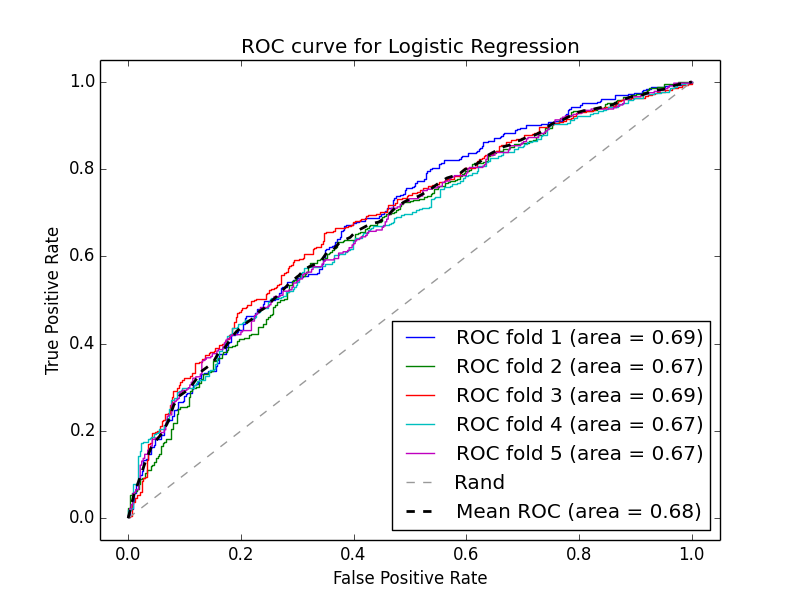
\includegraphics[scale=0.5]{Q1/ROC.png}
        		  }
    		\end{minipage}
	\item Give the AUC score (say AUC is the area under the ROC curve) \\
		0.68 as shown in the figure.
	\end{enumerate}
%% e %%
\item \ \\
	The null hypothesis is that logistic regression has the same F1 score with NBC , and the p-value of F1-score between logistic regression and NBC is 0.19062380751022309 > $\alpha = 0.05$. Therefore, we cannot reject the null hypothesis. \\
	The null hypothesis is that logistic regression has the same F1 score with linear SVM and the p-value of F1-score between logistic regression and linear SVM is 1.9670734624844568e-12 < $\alpha = 0.05$. Therefore, we can say that there is significant difference that logistic regression is better than linear SVM. \\
	The null hypothesis is that logistic regression has the same F1 score with Gaussian SVM and the p-value of F1-score between logistic regression and Gaussian SVM is 4.3700619261450163e-06 < $\alpha = 0.05$. Therefore, we can say that there is significant difference that logistic regression is better than Gaussian SVM. \\
%% f %%
\item \ \\
	I select the logistic regression as my algorithm and choose 'Interest Rate Percentage', 'Loan Purpose', 'Monthly PAYMENT', 'Debt-To-Income Ratio Percentage', 'FICO Range' as my features.
\end{enumerate}
\end{homeworkProblem}
\clearpage
%----------------------------------------------------------------------------------------
%	PROBLEM 2
%----------------------------------------------------------------------------------------

\begin{homeworkProblem}
\begin{enumerate}[a.]
\item \ \\
	\begin{enumerate}[1.]
		\item Shortest Path \\
		Since we are given the undirected graph $G_0$, for each node with more than 10 neighbors, we apply shortest path algorithm to find the nearest node that is not its neighbor and predict the edge between them as the missing edge. \\
		Advantage:\\
		\-\hspace{5mm}Based on existing algorithm and it is intuitive. \\
		
		Disadvantage:\\
		\-\hspace{5mm}Network diameter often very small and distribution very concentrated.\\
		
		\item Common Neighbors \\
		Common neighbors usess as score the number of common neighbors between vertices u and v. For each node with more than 10 neighbors, we calculate the score between the node and others that is not its neighbor to predict the one with highest score as missing edge.
		\begin{align}
		score(u,v) = |N(u) \cap N(v)|
		\end{align}
		Advantage: \\
		\-\hspace{5mm}The algorithm is efficient and works well on small society community. \\
		
		Disadvantage:\\
		\-\hspace{5mm}Large scores for vertices with too many neighbors \\	
		
		\item Jaccard Similarity \\
		The Jaccard Similarity is aimed to compensate the problem in Common Neighbors. It has same idea with Common Neighbors but with modified formula:
		\begin{align}
		score(u,v) = \frac{|N(u) \cap N(v)|}{|N(u) \cup N(v)|}
		\end{align}
		Advantage: \\
		\-\hspace{5mm}Fixes the issue of Common Neighbors, "u or v have too many neighbors", by dividing the intersection by the union. \\
		
		Disadvantage: \\
		\-\hspace{5mm}Although u, v are not problem, but the method fails to measure the quality of their neighbors. \\
		
		 \item Adamic / Adar \\
		 It is improved version of Jaccard Similarity and can be applied similarly as previous two methods, the formula it use is:
		 \begin{align}
		 score(u,v) = \sum_{z \epsilon N(u) \cap N(v)}\frac{1}{log|N(z)|}
		 \end{align}
		 where N(z) is the neighbors of the common neighbors of u and v. \\
		 Advantage: \\
		 \-\hspace{5mm}This score gives more weight to neighbors that are not shared with many others.
		 
		 Disadvantage: \\
		 \-\hspace{5mm}It is based on the hypothesis that the neighbor of u and v with less neighbors imply that u and v should know each other, which may not be true is some cases. \\
		 
		 \item Katz score \\
		 In Katz score, we calculate the score to find out the missing edges. The Katz score uses adjacency matrix A in its formula:
		 \begin{align}
		 score(u,v) = \sum_{l=1}^{\infty}\alpha^l(A^l)_{u,v}
		 \end{align}
		 The $\alpha$ is to ensure that the sum isn't divergent. \\
		 Advantage: \\
		 \-\hspace{5mm}The adjacency matrix A is easy to express the relationship between nodes.  A itself expresses the nodes with path of length 1 and  AA can express the number of common neighbors between $node_{i}$ and $node_{j}$. \\
		 
		 Disadvantage:\\
		 \-\hspace{5mm}For $\alpha << 1$, predictions will be approximated to common neighbors, which share the same defect. \\
		 
		 \item Page Rank \\
		 Each edge's vote is proportional to the importance of its source node. Therefore, if node j with importance $r_j$ has n out-edges, each link gets $\frac{r_j}{n}$ votes. Node j's own importance is the sum of the votes on its in-links.\\
		 For the stochastic adjacency matrix M, let node i has $d_i$ out-links. If $i\rightarrow j$, then $M_{ji} = \frac{1}{d_i}$ else $M_{ji} = 0$, where M is a colum stochastic matrix and the columns sum to 1. \\
		 Rank vector r: vector with an entry per page\\
		 $r_i$ is the importance score of node i and $\sum_ir_i=1$
		 Then the flow equations can be written as:
		 \begin{align}
		 r &= M \cdot r \\
		 (r_j  &= \sum_{i \rightarrow j}\frac{r_i}{d_i})
		 \end{align}
		 The pagerank also has random teleports to solve dead ends and spider trap problem, the modified formula is:
		 \begin{align}
		 r_j = \sum_{i\rightarrow j}\beta\frac{r_i}{d_i} + (1-\beta)\frac{1}{N}
		 \end{align}
		 In order to use pagerank to do link prediction, we have to apply rooted pagerank, which is also called personalized pagerank. The idea is based on hitting time . We first choose a rooted node say x, then for each step, there is $\alpha$ probability that goes back to x ('reset'), and there is $1-\alpha$ probability that goes from current node to its random neighbor. So the formula becomes:
		 \begin{align}
		 r_{root} &= \sum_{i\rightarrow j}\beta\frac{r_i}{d_i} + (1-\beta) \\
		 r_j &= \sum_{i\rightarrow j}\beta\frac{r_i}{d_i} \ ,\ \ \text{where}\ j\ !=\ root
		 \end{align}
		For each node, we use it as root to calculate its pagerank and retrieve the top 5 score nodes that is original not the neighbor of root as its missing neighbor.\\
		
		Advantage: \\
		\-\hspace{5mm} The matrix will always converge, so we don't need $\alpha$ value as in Katz score to prevent divergent.
		
		Disadvantage:\\
		\-\hspace{5mm} It share the same idea as hitting time and it is a randomized algorithm. Therefore, it relies on the probabilistic and may get bad result in chance.
		
	\end{enumerate}
\item \ \\
	In this question, I choose rooted pagerank as my best algorithm for it is well developed and efficient. To verify this approach, I randomly remove an edge from nodes with more than 10 edges and put those edges into validation set. By this way, I can test the prediction accuracy in my approach. For each node we report five candidates and if any of the candidate is the node of the removed edge, we view it as a successful hit. After comparing the accuracy of different methods, we select rooted pagerank as the best algorithm.\\ \\
	Then I put those edges back and re-run the algorithm to report the real missing candidate. \\ \\
	The data contains more than ten thousand nodes with approximate four thousand nodes with more than 10 edges. Each one hundred rooted pagerank procedure takes about three minutes. Therefore, to calculate all the four thousand nodes, it takes us about two hours.  \\ \\
	
	
\end{enumerate}
\end{homeworkProblem}
\clearpage
%----------------------------------------------------------------------------------------
%reference
%http://www.cs.cmu.edu/~tom/mlbook/NBayesLogReg.pdf
%http://web.engr.oregonstate.edu/~xfern/classes/cs534/notes/logistic-regression-note.pdf

\end{document}